\subsection{Static PageRank}

PageRank~\cite{page} is computed on a graph $G(V, E, w)$ where $V$ ($n = |V|$) is the set of vertices representing the web pages, $E$ ($m = |E|$) is the set of edges representing the hyperlinks, and $w$ is the set of edge weights which represent the \emph{contribution} of a vertex to the vertex it connects with via an edge. Using the random-surfer model, which accounts for any random internet user to land at a particular page, the rank of a vertex $v$ is given as:

\begin{equation}
\label{eq:pr1}
    pr_v = \sum_{u \in in_v} c_{u \rightarrow v} + \frac{1 - d}{n}
\end{equation}

In Equation~\ref{eq:pr1}, $d$ is the \emph{damping factor} (taken as $0.15$ conventionally), which represents the probability of a random surfer jumping to a random page on the internet, instead of following one of the links on the given page. The function $c_{u \rightarrow v}$ is the contribution of PageRank score from a page $u$ pointing to the given page $v$. Its magnitude is proportional to the PageRank score of the pointing page ($u$) $pr_u$, and is inversely proportional to the degree of the pointing page ($u$) $outdeg_u$, such that the total value of contributions from $u$ never exceeds its own rank $pr_u$. It is expressed as:

\begin{equation}
\label{eq:pr2}
c_{u \rightarrow v} = (1 - d) \times  \frac{pr_u}{outdeg_u}
\end{equation}

For static PageRank computation (from scratch) we will refer to baseline algorithm as discussed in Garg et al.~\cite{pr-sticd16}. At the beginning they consider PageRank score to be $d/n$ where $d$ is damping factor and $n$ is number of vertices. Furthermore, they compute new PageRank of every vertex considering the contribution provided by its incoming neighbours.

In Equation~\ref{eq:pr2}, we observe that PageRank computations can happen via cyclic contributions of two vertices on each other. Thus, PageRank values are iteratively computed for all vertices until they converge. This signifies that there are small updates to the scores after a particular iteration. This style of computing PageRank scores is popularly done through \emph{power iterations}~\cite{page}. Power iterations arises from the idea of modeling the computations of the PageRank scores as a Markov chain that reaches a steady state when starting from an initial distribution. Here, the initial scores compose the starting states of every vertex which then go through several transitions to reach a stable state. The scores of all the vertices can be arranged to form a distribution (or transition) matrix which has a set of eigenvalues. The eigen vectors of the said state matrix is solved using power iterations. By the intrinsic property of Markov chains, if the state matrix is stochastic, aperiodic, and irreducible, then the state matrix will converge to a stationary set of vectors which will be the final scores. Monolithic PageRank, as referred to here, is a \emph{pull-based} standard power-iteration approach \cite{pr-whang15}, where all vertices in the graphs are processed in each iteration.

\begin{algorithm}[!hbtp]
\caption{Algorithm for computing \emph{static PageRank} (static Monolithic). Here, $G$ is the current snapshot of the graph.}
\label{alg:static}
\begin{algorithmic}
% \Require{$G$: Graph (V, E)}
\Function{staticPR}{$\vars{G}$}
\State $V \gets G.vertices$
\State $n \gets G.order$
\ForAll{$u \in V$} \textbf{in parallel}
  \State $prev_u = 1/n$
\EndFor
\Return{$\textsc{monolithicLoop}(G, [V], prev)$}
\EndFunction

\Statex

\Function{monolithicLoop}{$\vars{G}, \vars{SCCs}, \vars{prev}$}
  \State $MAX\_ITERS \gets 500$
  \State $\tau \gets TOLERANCE = 10^{-6}$
  \ForAll{$l \in range(0, MAX\_ITERS)$}
    \State $pr \gets \textsc{calculateRanks}(G, SCCs, prev)$
    \If{$l\infty{}Norm(prev, pr) < \tau$}
        \State $\textrm{break}$
    \EndIf
    \State $prev \gets pr$
  \EndFor
  \Return{$pr$}
\EndFunction

\Statex

\Function{calculateRanks}{$\vars{G}, \vars{SCCs}, \vars{prev}$}:
  \State $d \gets DAMPING = 0.15$
  \State $n \gets G.order$
  \State $outdeg \gets G.outDegrees$
  \ForAll{$SCC \in SCCs$} \textbf{in parallel}
    \ForAll{$v \in SCC$} \textbf{in parallel}
      \State $pr_v = d/n + (1 - d) * \Sigma _{u \in in(v)} \frac{prev_u}{outdeg_u}$
    \EndFor
  \EndFor
  \Return{$pr$}
\EndFunction
\end{algorithmic}
\end{algorithm}





\subsection{STIC-D PageRank}

Garg and Kothapalli \cite{pr-sticd16} rearrange the computation of PageRank as a level ordered computation. The computation of PageRank using the algorithm of Garg and Kothapalli \cite{pr-sticd16} works as follows. They first observe that the input directed graph $G$ can be partitioned into SCCs. These SCCs can be also be arranged into a block-graph $\gscc$ where each SCC of $G$ is a vertex in $\gscc$ and a directed edge is added to two vertices $u$ and $v$ in $\gscc$ if there is an edge from some vertex $x$ in the SCC $C_u$ in $G$ corresponding to $u$ (in $\gscc$) to a vertex $y$ in the SCC $C_v$ in $G$ corresponding to $v$ (in $\gscc$). The graph $\gscc$ is a directed acyclic graph. Hence, the vertices of $\gscc$ can be arranged into levels numbered 0, 1, 2, $\cdots$, such that vertices in a level $\ell$ have directed edges coming in only from vertices in a level numbered at most $\ell$ and have directed edges to vertices in a level numbered at least $\ell$. Such a level-wise ordering of SCCs imposes a \emph{dependency relation} between SCCs. PageRank computation on each SCC is then performed in the \emph{topological order} of each SCC in the block-graph, until it converges. An SCC can only be processed after all the SCCs it is dependent upon, as indicated by incoming edges in the block-graph, have converged. This dependency relation between SCCs is what allows for the ranks of independent SCCs to be computed separately, in a distributed manner. SCCs of the given graph are obtained in the preprocessing stage. In addition, the algorithm from \cite{pr-sticd16} introduces other optimizations such as those corresponding to removal of identical vertices, chain vertices, and dead vertices, which help in faster computation of PageRanks.

\begin{figure}[!hbtp]
  \centering  % \vspace{-0.3 cm}
  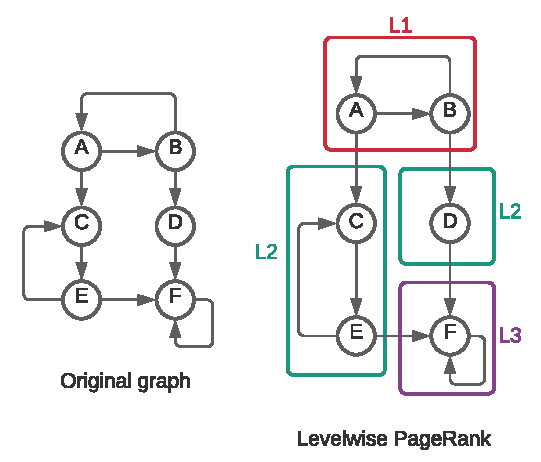
\includegraphics[width=0.48\textwidth]{out/about-levelwise.pdf}
  \caption{Consider a graph with 6 vertices, as shown on the left. This graph has 4 SCCs, C1 with vertices A and B, C2 with vertices C and E, C3 with vertex D, and C4 with vertex F. Its block-graph consists of vertex C1 pointing to C2, which then points to C3. This is the order in which SCCs are processed as per the \levelwisePR{} algorithm.}
  \label{fig:levelwise}
\end{figure}

\begin{algorithm}[!hbtp]
\caption{Algorithm for computing \emph{plain STIC-D PageRank} (static Levelwise) without identical, chain, and dead vertex optimizations. Here, $G$ is the current snapshot of the graph.}
\label{alg:sticd}
\begin{algorithmic}
% \Require{$G$: Graph (V, E)}
\Require{$SCC+TOPO(G)$: finds components of $G$ in topological order grouped by levels in block-graph}
\Function{sticdPR}{$\vars{G}$}
\State $[[C_{11}, C_{12}, \cdots], \cdots] \gets SCC{+}TOPO(G)$
\ForAll{$u \in V$}
  \State $pr_u = 1/n$
\EndFor
\ForAll{$i \in range(0, levels)$}
  \ForAll{$C_{ij} \in [C_{i1}, C_{i2}, \cdots]$} \textbf{in parallel}
    \State $pr \gets \textsc{calculateRanks}(G, [C_{ij}], pr)$ \\ \Comment{see Algorithm \ref{alg:static}}
  \EndFor
\EndFor
\Return{$pr$}
\EndFunction
\end{algorithmic}
\end{algorithm}





\subsection{nvGraph PageRank}

The NVIDIA Graph Analytics library (nvGraph)~\cite{pr-nvgraph} is a library of high performance parallel graph algorithms. It has been designed keeping the core functionality of all graph operations centered around sparse linear algebra. The library provides graph construction and manipulation primitives that are optimized for NVIDIA GPUs. It also provides optimized implementations for the core computation of sparse matrix vector products using a semi-ring model, with automatic load balancing for any sparse pattern. The library is currently distributed as a part of the larger RAPIDS framework and contains implementations for a wide range of traditional graph processing algorithms like community detection, shortest paths, link analysis, connected components, and flow. It has support for three different graph storage formats: Compressed Sparse Row (CSR), Compressed Sparse Column (CSC), and the Coordinate list (COO). The library also allows a program to extract a subgraph based on the list of vertices or list of edges. 




%\textbf{Spider traps} are groups of vertices (or even just a single vertex) which \emph{only out-link each other}. Eventually, spider traps absorb all the \emph{importance} and such vertices delay or hamper the PageRank calculation. A solution to this issue is to use a \emph{damping factor $\alpha$} (also called \emph{taxation}), which controls the probability with which the surfer follows one of the links on a given page \cite{pr-kang}. It is usually set to \emph{0.85}. Which means there is a \emph{15\% chance} of the surfer teleporting to a random page at any time.
%On the other hand, \textbf{dead ends} (or \emph{dangling vertices}) are vertices which have \emph{no out-links}. This means the random-surfer has \emph{nowhere} to go. In the presence of such web pages (vertices), the \emph{probability transition matrix} is not \emph{column stochastic}, which is a \emph{requirement} for \kk{PageRanks to converge.} Several authors suggest different ways to handle this scenario, including  teleport  \cite{pr-deeper01,pr-kang},  adding self loops to such vertices or all vertices, or removing all dead ends recursively. The PageRanks obtained do differ based on the strategy employed to deal with dead ends.
% \emph{Markov chains}. This can cause \emph{importance} to \emph{leak out} of the graph. The most commonly used solution to this is to allow the surfer to \emph{always} \textbf{teleport} to a random page upon reaching a \emph{dead end} \cite{pr-deeper01, pr-kang}. This however, is \emph{not} an ideal strategy for handling dead ends with \emph{dynamic PageRank} since any \emph{affected dead end (including dead ends in the previous snapshot)} can affect the ranks of \emph{all vertices} in the graph. Note that, \emph{affected vertices} are those which are either \emph{changed vertices}, or are \emph{reachable} from changed vertices. \emph{Changed vertices} are those which have an edge added or removed between it and another (changed) vertex.
%Other possible strategies of \textbf{handling dead ends} include \emph{adding self loops to dead ends} (used here), \emph{adding self loops to all vertices}, or even \emph{removing all dead ends recursively} (as removing existing dead ends can introduce new dead ends). None of these require a \emph{common teleport contribution} calculation per iteration, or enable a single affected vertex to affect ranks of all vertices (unlike \emph{teleport} strategy). It important to note however that \emph{ranks} obtained with the use of each such dead-end handling strategies can be \emph{significantly} different, because of their semantic difference.


% A \emph{block-graph} is then obtained, where each \emph{vertex} in the \emph{block-graph} denotes an \emph{SCC} in the \emph{original graph}, and the \emph{edges} represent \emph{cross-edges between SCCs}.  


%\kk{Move this to Preliminaries. Talking about Levelwise/Monolithic at this stage is premature. \textbf{Levelwise PageRank} is one such technique for the PageRank algorithm. It decomposes the input graph into a directed acyclic block-graph of strongly connected components, and processes them in topological order, one level at a time \cite{pr-sticd16}. It enables one to perform PageRank computation in a \textit{distributed fashion} \textbf{without per-iteration communication}. In contrast, the standard method of PageRank computation requires all vertices in the graph to be processed in each iteration, and performing it in a distributed manner would require communicating ranks of vertices between processors in every iteration. It should however be noted that this technique can \textit{only} be applied on graphs \textit{without dead ends} (discussed in detail later).}
%\su{Ok sir but i was thinking of explaining the motivation of the paper right in the first paragraph.}
% (vertices with no outgoing edges, also commonly called dangling vertices). This is discussed in detail later. However, this is usually a non-issue as they can be dealt with by adding self-loops to such vertices. Other possible alternatives include adding self-loops to all the vertices, or even removing all dead ends recursively (as removing existing dead ends can introduce new dead ends). It is also important to note that ranks obtained with the use of each such dead-end handling strategies can be significantly different, because of the semantic difference between each strategy.


% \kk{Subhajit: The discussion on monolithic and levelwise will go to the next section on algorithmic details.}
% \su{Sir, i wrote about monolithic and levelwise in preliminaries to include details already known before this paper. Such as for monolithic is discuss the standard approach for computing PageRank where all vertices are processed. Similarly with levelwise is write about the algorithm published by paritosh in 2016. In the algorithmic approaches section i only then include new modifications to each algorithm.}
